\section{Data and simulated samples}\label{chap5:dataset}

Data recorded in proton proton collisions at 13\TeV during 2015 was used in the analysis, with a total integrated luminosity of 2.3\ifb. Single  and double lepton triggers are used similarly to the same analysis at 8\TeV. The HLT paths and descriptions of the triggers used in this analysis are described in Tables~\ref{table:ele_trigg_13} and ~\ref{table:mu_trigg_13} for electrons and muons respectively.

\begin{table}[h]
\caption{HLT paths related to Electrons}
\label{table:ele_trigg_13}
\scalebox{0.75}{
\begin{tabular}{ll}
\hline
HLT Path & Description \\
\hline\hline
HLT\_Ele23\_WPLoose\_Gsf\_v*   &
\parbox{11cm}{$\,$ \\Single Electron trigger. Best trigger to be used for 2015 data. In HWW, we are using ``Trigger safe'' Id. Turn on is at around Ele $\rm p_{T}$ = 30 GeV\\}\\
\hline
HLT\_Ele17\_Ele12\_CaloIdL\_TrackIdL\_IsoVL\_DZ\_v* &
\parbox{11cm}{$\,$ \\Double Electron Trigger. Best trigger to cover the turn on region from single electron trigger. ``DZ'' filter is also present. Its efficiency is also calculated separately.}\\
\hline
HLT\_Ele12\_CaloIdL\_TrackIdL\_IsoVL\_v* &
\parbox{11cm}{$\,$ \\This electron leg of \\
HLT\_Mu17\_TrkIsoVVL\_Ele12\_CaloIdL\_TrackIdL\_IsoVL\_v*\\
same as Ele12 leg of double electron trigger.\\} \\
\hline
HLT\_Ele17\_CaloIdL\_TrackIdL\_IsoVL\_v*&
\parbox{11cm}{$\,$ \\This electron leg of\\
HLT\_Mu8\_TrkIsoVVL\_Ele17\_CaloIdL\_TrackIdL\_IsoVL\_v* \\
same as Ele17 leg of double electron trigger.} \\
\hline
\end{tabular}
}
\end{table}

\begin{table}
\caption{Muon trigger's elements description}
\label{table:mu_trigg_13}
\scalebox{0.8}{
\begin{tabular}{ll}
\hline
HLT path \\
\hline\hline
HLT\_IsoMu18\_v*   & 
\parbox{11cm}{$\,$ \\single muon trigger\\}\\
\hline
HLT\_IsoTrMu20\_v* &
\parbox{11cm}{$\,$ \\single muon trigger with tracker isolation\\}\\
\hline
HLT\_Mu17\_TrkIsoVVL & 
\parbox{11cm}{$\,$ \\leg for the HLT\_Mu17\_TrkIsoVVL\_Mu8\_TrkIsoVVL\_DZ\_v*,\\
HLT\_Mu17\_TrkIsoVVL\_TkMu8\_TrkIsoVVL\_DZ\_v* and\\ 
HLT\_Mu17\_TrkIsoVVL\_Ele12\_CaloIdL\_TrackIdL\_IsoVL\_v*\\
double lepton triggers\\} \\
\hline
HLT\_Mu8\_TrkIsoVVL &
\parbox{11cm}{$\,$ \\leg for the HLT\_Mu17\_TrkIsoVVL\_Mu8\_TrkIsoVVL\_DZ\_v* and\\
HLT\_Mu8\_TrkIsoVVL\_Ele17\_CaloIdL\_TrackIdL\_IsoVL\_v* \\ 
double lepton triggers\\} \\
\hline
HLT\_TkMu8\_TrkIsoVVL &
\parbox{11cm}{$\,$ \\leg for the HLT\_Mu17\_TrkIsoVVL\_TkMu8\_TrkIsoVVL\_DZ\_v*\\
double muon trigger\\} \\
\hline
$DZ_{\mu\mu}$ &
\parbox{11cm}{$\,$ \\efficiency of DZ cut in \\
the HLT\_Mu17\_TrkIsoVVL\_Mu8\_TrkIsoVVL\_DZ\_v*\\
and HLT\_Mu17\_TrkIsoVVL\_TkMu8\_TrkIsoVVL\_DZ\_v* \\
double muon triggers, it is around 95\%\\} \\
\hline
\end{tabular}
}
\end{table}

The trigger efficiencies are measured in data and applied on simulated events as described in Sec.~\ref{subsec:Datasets}.


%Monte Carlo
Concerning the simulated samples, several different Monte Carlo (MC) generators were used. 
In the simulation, `lepton' includes also $\tau$.
Higgs signal samples have been simulated in all channels with
\textsc{Powheg v2}~\cite{Nason:2004rx,Frixione:2007vw,Alioli:2010xd}, designed to describe the full NLO properties of these processes.
In particular, for Higgs produced via gluon fusion~\cite{Alioli:2008tz}, and vector-boson-fusion (VBF)~\cite{Nason:2009ai},
the decay of the Higgs boson into two W boson and subsequently into leptons was done using \textsc{JHUGen} v5.2.5~\cite{JHUGen}. 
For associated production with a vector boson ($\mathrm{W}^{+}\mathrm{H}$, $\mathrm{W}^{-}\mathrm{H}$, ZH)~\cite{Luisoni:2013kna}, including gluon fusion produced ZH (ggZH), 
the Higgs decay was done via \textsc{pythia} 8.1~\cite{Sjostrand:2007gs}.  Alternative signal samples were produced with \textsc{aMC@NLO}~\cite{Alwall:2014hca}, or  with \textsc{Powheg v2} but decayed via \textsc{pythia} 8.1 for gluon fusion and VBF assuming 
a Higgs boson mass of 125\GeV. In the following, the mass of the SM Higgs boson is assumed to be 125\GeV.

The WW production, irreducible background for the analysis, was simulated in different ways. 
\textsc{Powheg v2}~\cite{Melia:2011tj} was used for $\mathrm{q\bar q}$ produced WW in different decays. 
The cross section used for normalizing WW processes produced via $\mathrm{q\bar q}$ was computed at next-to-next-to-leading order (NNLO)~\cite{Gehrmann:2014fva}. 
In order to control the top quark background processes, the analysis is performed with events that have no more than one 
high-\pt jet. The veto on high-\pt jets enhances the importance of logarithms of the jet \pt, spoiling the convergence of 
fixed-order calculations of the qq$\rightarrow$WW process and requiring the use of dedicated resummation techniques for an
accurate prediction of differential distributions~\cite{Meade:2014fca,Jaiswal:2014yba}. 
The \pt of the jets produced in association with the WW system is strongly correlated with its transverse momentum, 
$\pt^\mathrm{WW}$, especially in the case where only one jet is produced. The simulated qq$\rightarrow$WW events are reweighted  
to reproduce the $\pt^\mathrm{WW}$ distribution from the \pt-resummed calculation.

Gluon fusion produced WW was generated, with and without Higgs diagrams, using \textsc{mcfm} v7.0~\cite{Campbell:2013wga}. 
A \ttbar sample dilepton sample was also generated using \textsc{Powheg v2}. The WW and \ttbar samples 
produced specifically for this analysis are presented in Table~\ref{tab:wwl}.

\begin{table*}[htbH]
\caption{Simulated samples for \ttbar and \WW production. The $gg\rightarrow$\WW$\rightarrow2\ell2\nu$ (H diagr.) sample includes both 
ggH production, the ggWW component and the interference.}\label{tab:wwl}
\begin{center}
\begin{tabular}{lc}
\hline
Process & $\sigma\times\mathcal{B}$ [\pb] \\
\hline
\hline
\ttbar$\rightarrow$\WW$b\bar{b}\rightarrow2l2\nu b\bar{b}$ & 87.31 \\
$\mathrm{q\bar q}\rightarrow$\WW$\rightarrow2l2\nu$ & 12.178 \\
$gg\rightarrow$\WW$\rightarrow2l2\nu$ & 0.5905 \\
$gg\rightarrow$\WW$\rightarrow2l2\nu$ (H diagr.) & 0.9544\\
\hline

\end{tabular}
\end{center}
\end{table*}


Additional gluon fusion and VBF samples covering a large Higgs mass range, from 115 to 1000\GeV,
were produced using \textsc{Powheg v2}, and the decay of the Higgs boson was done via \textsc{JHUGen} v6.2.8.

Other background samples are used, a list of the most relevant ones is presented in Table~\ref{tab:otherbck}.


\begin{table*}[htbH]
\caption{Simulated samples for other backgrounds used in the analysis.\label{tab:otherbck}}
\begin{center}
\begin{tabular}{lc}
\hline
Process & $\sigma\times\mathcal{B}$ [\pb] \\
\hline\hline
Single top &   71.7  \\
Drell-Yan ($10\GeV < \mll < 50\GeV$)  &  20471.0  \\
Drell-Yan ($\mll > 50\GeV$)   &  6025.26  \\
WZ$\to2\ell2\mathrm{q}$ &  5.5950 \\
ZZ$\to2\ell2\mathrm{q}$ &  3.2210 \\
WWZ &  0.1651 \\
WZZ &  0.05565 \\
ZZZ &  0.01398  \\
\hline
\end{tabular}
\end{center}
\end{table*}

All processes are generated using the NNPDF2.3~\cite{Ball:2013hta,Ball:2011uy} parton distribution functions (PDF) for NLO generators,
while the LO version of the same PDF is used for LO generators. All the event generators are interfaced 
to \textsc{pythia} 8.1~\cite{Sjostrand:2007gs} for the showering of
partons and hadronization, as well as including a simulation of the underlying event (UE) and multiple interaction (MPI)
based on the CUET8PM1 tune~\cite{Khachatryan:2015pea}. 
%
To estimate the systematic uncertainties related to the choice of UE and MPI tune, the signal processes and the WW
events are also generated with two alternative tunes which are representative of the errors on the tuning parameters.
The showering and hadronization systematic uncertainty is estimated by interfacing the same MC samples with the 
\textsc{herwig ++} 2.7 parton shower~\cite{Richardson:2013nfo,Bellm:2013hwb}.
%
For all processes, the detector response is simulated using a detailed
description of the CMS detector, based on the \textsc{geant4} package~\cite{Agostinelli:2002hh}. 

%PU
The simulated samples are generated with distributions for the number of pileup interactions that are meant to roughly cover,
though not exactly match, the conditions expected for the different data-taking periods. In order to factorize these effects, 
the number of true pileup interactions from the simulation truth is reweighted to match the data.
The re-weighting is propagated automatically to both the in-time pile up and the out-of-time one.
In Fig.~\ref{Fig:pu}, the effect of this reweighting on a sample enriched in Drell-Yan events is shown.
Before the reweighting the simulation is presented in the open red histogram; after the reweighting,
it is represented by the solid green histogram that matched well the data. In order to select this sample, 
events with two leptons with \pt$> 20$\GeV, opposite sign, and same flavour, are selected only if  $|\mll - m_\mathrm{Z}| < 15$\GeV. 

\begin{figure*}[htbp]
\centering
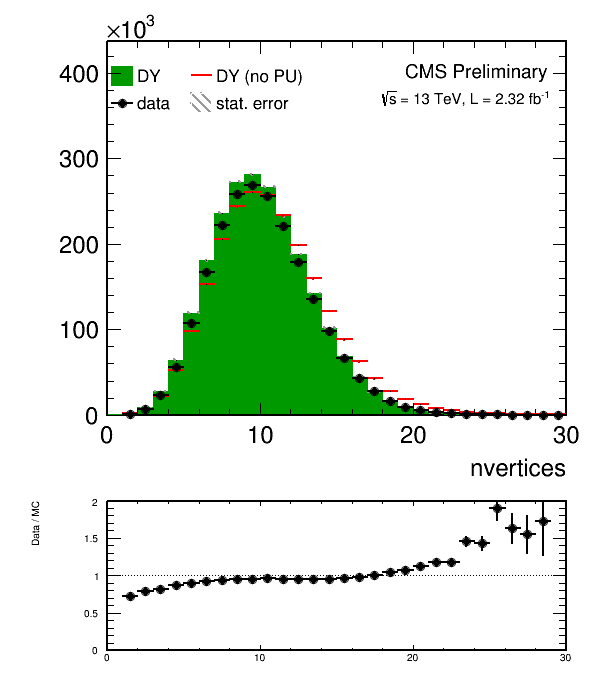
\includegraphics[width=0.45\textwidth]{images/13TeV/nvertices.png}
\caption{
    Distributions of the number of vertices in a Drell-Yan enriched sample in data,
    together with the simulation before (red) and after (solid green) the pileup reweighting. }
    \label{Fig:pu}
\end{figure*}

The average number of pileup is approximately 11.5.


%Cross sections
Different sources and calculations are used to obtain the cross sections for the different processes at 13\TeV. 
For Higgs signal, the cross sections used are the ones reported by the LHC Higgs Cross Section Working Group~\cite{temphiggsxsecs},
computed at NNLO and NNLL QCD and NLO EW for gluon fusion, and at NNLO QCD and NLO EW for the rest of the production modes.
The 	anching fractions are the ones reported in Ref.~\cite{Heinemeyer:2013tqa}. 

The cross section used for normalizing $\mathrm{q\bar q}$ produced WW processes was computed at next-to-next-to-leading order
(NNLO)~\cite{Gehrmann:2014fva}. The leading-order (LO) cross section for ggWW is obtained directly from \textsc{mcfm}.
For gluon fusion, the difference between LO and NNLO cross sections is significantly big.
A scale factor of 1.4 is theoretically calculated~\cite{Caola:2015rqy}. For the LO simulation of the interference between 
gg$\rightarrow$WW and gluon fusion  produced H$\rightarrow$WW a k-factor of 1.87 is applied. 
This k-factor is obtained as the average between LO to NNLO ggH scale factor and LO to NLO ggWW scale factor 
(from private communication with the authors of~\cite{Caola:2015rqy}). 

The cross sections of the different single top processes are estimated by the LHC Top Working group~\cite{singletop} at NLO.
The \ttbar cross section is also provided by the LHC Top Working group~\cite{topxsec}, and it is computed at NNLO, with NNLL soft gluon resummation. 

Drell-Yan (DY) production of Z/$\gamma^{*}$ is generated using \textsc{aMC@NLO}~\cite{Alwall:2014hca}. 
Other multiboson processes, such as WZ,ZZ, and VVV (V=W/Z), are generated with \textsc{aMC@NLO} and normalized
to the cross section obtained at NLO in generation.

All processes are generated using the NNPDF2.3~\cite{Ball:2013hta,Ball:2011uy} parton distribution functions (PDF) for NLO generators,
while the LO version of the same PDF is used for LO generators. All the event generators are interfaced 
to \textsc{pythia} 8.1 for the showering of partons and hadronization, as well as including a simulation of the 
underlying event (UE) and multiple interaction (MPI) based on the CUET8PM1 tune~\cite{Khachatryan:2015pea}. 
